
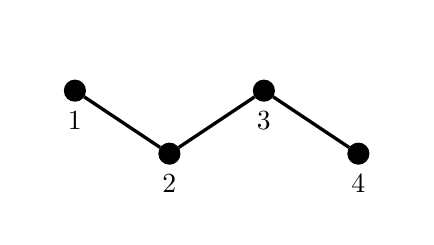
\begin{tikzpicture}[
    x = 1.2cm,
    y = 0.8cm,
    scale=1,
    >=stealth,
    atom/.style = {circle, fill=black, minimum size=8pt,
              inner sep=0pt, outer sep=0pt},
    ]

\node[atom, label=below:1] (atom_1) at (0,1){};
\node[atom, label=below:2] (atom_2) at (1,0){};
\node[atom, label=below:3] (atom_3) at (2,1){};
\node[atom, label=below:4] (atom_4) at (3,0){};
\draw [black, solid, very thick] (atom_1) -- (atom_2);
\draw [black, solid, very thick] (atom_2) -- (atom_3);
\draw [black, solid, very thick] (atom_3) -- (atom_4);
\clip (-0.5,-1) rectangle (3.5,2);

\end{tikzpicture}

